\documentclass[
  a4paper,
  12pt,
  oneside,
  parskip=half,
  listof=totoc,
  bibliography=totoc,
  DIV=12,
  numbers=noenddot,
  BA.tex
  ]{subfiles}

\begin{document}

\section{Event simulation: The identification of potential biases}
\label{sec:event-simulation}

This chapter introduces the simulation of Pb--Pb events, motivated by the search for potential mistakes in the diffusion wake analysis. It provides details on simulation parameters and data that is used. Then, the diffusion wake measurements in chapter \ref{sec:dianaALICE} are repeated with simulated Pb--Pb events. The simulation is then used to study how parameter changes on the simulation influence the diffusion wake analysis result.

\subsection{Motivation}

When conducting analyses in heavy ion physics or particle physics one usually has to select experimental data from a huge data collection. However, this data selection process is nontrivial and has obvious but also hidden consequences on the outcome of the analysis. In the following two examples are given to illustrate how certain selections can bias the result of a measurement. One would like to measure the average elliptic flow parameter $v_2$ in Pb--Pb collisions (see chapter \ref{sec:analysis-of-heavy-ion-collision-data} for an introduction to flow physics). For that a sample of Pb--Pb data in the centrality category of 0-10\% is used. A certain value for $v_2$ is the result. But this value is not representative for Pb--Pb collisions in general, because the cut on the most central events has removed all peripheral events from the analysis. Therefore, the value of $v_2$ in peripheral events is omitted in the analysis. This is called a selection bias. Another mistake that could happen in this analysis is to also take high-$p_T$ particles into account in the particle correlation from which the $v_2$ flow parameter is derived. This is incorrect, since high-$p_T$ particles as jet constituents are not subject to flow in the hydrodynamic calculation. One can see that such mistakes can be made in many stages of the analysis. To avoid those errors, a simulation can be used to crosscheck the analysis result. No diffusion wake signal should be seen when conducted with simulated data that does not simulate jet-hydrodynamic effects. On the other hand, if the simulated data analysis shows signals of the same kind and order of magnitude as the diffusion wake, it is possible that the very same effect took place in the real data analysis.

\subsection{Modeling the simulation}

Each simulated Pb--Pb event is an overlay of soft hadron background from the medium expansion and hadronization, and artificially generated jets from hard scatterings. Both components do not interfere with each other, meaning that the jets are not subject to jet quenching and the medium is not affected by the artificially inserted jets.

The thermal background will involve isotropic flow, that is the uniform distribution of particles in the $(\phi, \eta)$ phase space, but also anisotropic flow in the shape of directed, elliptic and triangular flow ($v_1, v_2, v_3 \neq 0$) for each particle. The background is generated based on characteristics of $0-10\%$ ALICE Pb--Pb data from the Run 2 period at $\sqrt{s_{NN}} = 5.02\bunit{TeV}$ \cite{nadine_alice_grunwald_studies_2022} and also $0-5\%$ ALICE Pb--Pb data at $\sqrt{s_{NN}} = 2.76\bunit{TeV}$ \cite{collaboration_pseudorapidity_2016}. The utilized 0--10\% statistics involve information on event-wise charged hadron multiplicity probability densities $p(N_\text{ch})$, track-wise transverse momentum probability densities $p(p_T)$ and also track-wise transverse momentum dependent elliptic flow parameter statistics $v_2(p_T)$. Because the $v_2(p_T)$ statistics also include higher-$p_T$ particles that are not subject to flow, it was corrected such that $\lim_{p_T \rightarrow \infty}  v_2(p_T) = 0$ by fitting an exponentially decaying function to the data points below $p_T \leq 5\unit{GeV/c}$. This value has been chosen because the logarithmic representation of the particle $p_T$ spectrum of Pb--Pb collisions shows an exponential decay according to Boltzmann statistics for $p_T \in [0, 5]\unit{GeV/c}$ (see figure \ref{fig:simulationinput}). Such low transverse momenta are therefore dominated by thermal particles that are subject to flow. For higher values this exponential decay gets distorted by hadrons from hard parton interactions and jets. The directed flow $v_1$ depends linearly on $\eta$, relevant data was taken from \cite{selyuzhenkov_charged_2011}. The elliptic flow of particles decreases with larger pseudorapidity, but the measured dependence of $v_2$ on $|\eta|$ is provided too coarse for mid-rapidity analyses\cite[Figure 1, $v_2\{2\}$ for 0--5\%,][]{collaboration_pseudorapidity_2016}. That is why it has been modeled with a linear fit empirically for data points that fulfill $|\eta| \leq 1.25$ to approximate the behavior at a pseudorapidity accessible to ALICE. Since $v_2(\eta)$ has only been measured globally for particles with a transverse momentum below $5\bunit{GeV/c}$, it is understood as a reduction factor. In practice the particle's individual $v_2(p_T)$ will be reduced by the fraction that $v_2(\eta)$ decreases relative to $\eta = 0$. The value of the triangular flow coefficient was chosen to be equal to the elliptic flow coefficient, that is $v_3(p_T, \eta) \equiv v_2(p_T, \eta)$. This was chosen as a simplification because the orders of magnitude of both values are the same \cite{alqahtani_understanding_2026}. The Fourier series expansion of the azimuthal particle transverse momentum correlation (see equation (\ref{eq:FourierExpansion})) is used to generate the particles' azimuthal coordinates. The definition of this expansion has the expressions $\cos(n(\phi - \psi_m))$ as base functions. A direct consequence of truncating the series after the third harmonic, as done in this simulation, is that fluctuations, embodied by $v_n |_{n \geq 3}$ are always aligned with the event plane (see figure \ref{fig:simuflow}). To avoid this, the offset angle of the triangular flow is defined randomly relative to the event plane angle. The resulting azimuthal particle correlation probability density is

\begin{equation}
	\label{eq:phi_prob_dist}
	p(\phi) = \frac{1}{2\pi} \left\{ 1 + 2 \left[v_1 \cos(\phi - \psi_m) +  v_2 \cos(2(\phi - \psi_m)) + v_3 \cos(3(\phi - \psi_3)) \right] \right\} \, .
\end{equation}


\begin{figure}[H]
	\centering
	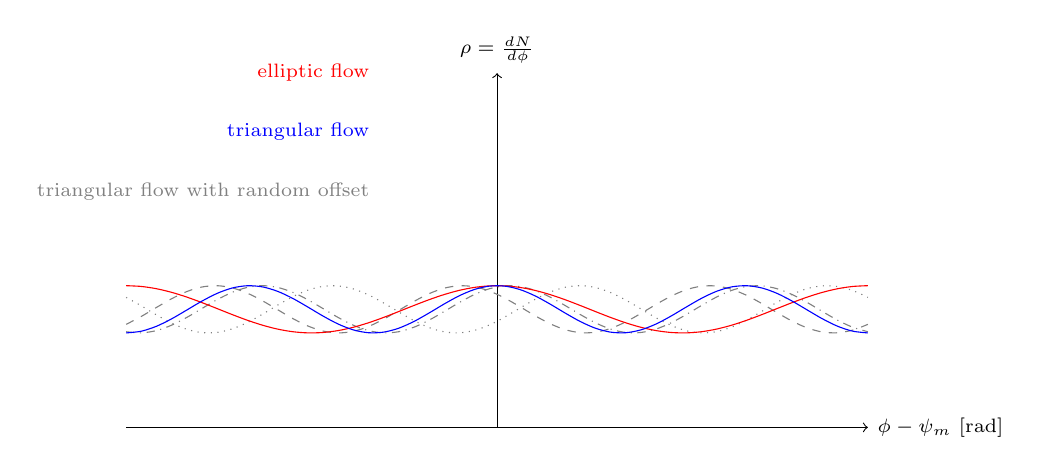
\begin{tikzpicture}[scale=1.5]
		%draw coordinate system
		\draw [->] (-3.14,0) -- (3.14,0)node[right] {\scriptsize $\phi - \psi_m$ [rad]};
		\draw [->] (0,0) -- (0,3) node[above] {\scriptsize $\rho = \frac{d N}{d \phi}$};
		%draw functions
		\draw [gray, dotted] plot[domain=-3.14:3.14,
		samples = 50,
		smooth]({\x}, {1 + 0.2*cos((360/6.28)*3*(\x-.7))});
		\draw [gray, dashed] plot[domain=-3.14:3.14,
		samples = 50,
		smooth]({\x}, {1 + 0.2*cos((360/6.28)*3*(\x-1.8))});
		\draw [gray, dash dot] plot[domain=-3.14:3.14,
		samples = 50,
		smooth]({\x}, {1 + 0.2*cos((360/6.28)*3*(\x-2.2))});
		\draw [red] plot[domain=-3.14:3.14,
		samples = 50,
		smooth]({\x}, {1 + 0.2*cos((360/6.28)*2*\x)});
		\draw [blue] plot[domain=-3.14:3.14,
		samples = 50,
		smooth]({\x}, {1 + 0.2*cos((360/6.28)*3*\x)});
		%draw labels
		\draw (-1,3) node[color=red, anchor=east] {\scriptsize elliptic flow};
		\draw (-1,2.5) node[color=blue, anchor=east] {\scriptsize triangular flow};
		\draw (-1,2.0) node[color=gray, anchor=east] {\scriptsize triangular flow with random offset};
		
	\end{tikzpicture}
	\caption{The soft hadron correlation with the event plane that has azimuthal angle $\psi_m$. The elliptic flow (red) defines the event plane and is therefore always aligned with the event plane. The triangular flow (blue) in the Fourier expansion definition is also aligned with the event plane. The modified definition of the triangular flow (gray) makes the simulation of fluctuations possible.}
	\label{fig:simuflow}
\end{figure}


A collection of the statistics that are used to simulate the thermal background are shown in figure \ref{fig:simulationinput}. Fit functions used for interpolating the pseudorapidity and transverse momentum dependence of the flow parameters are 

\begin{figure}
	\centering
	\includegraphics[width=\textwidth]{Media/Plots/SimulationInputs.pdf}
	\caption{The statistics that are used for Monte Carlo generating the thermal particle background showing (from top to bottom) the per-event multiplicity probability density $p(N)$, the per-particle transverse momentum probability density $p(p_T)$, the per-particle elliptic flow parameter $v_2(p_T)$ depending on its transverse momentum and the per-particle flow parameters $v_1(\eta),v_2(\eta)$ depending on pseudorapidity. The data from the first three plots was extracted from \cite{nadine_alice_grunwald_studies_2022}. The data for the fourth plot was extracted from \cite{collaboration_pseudorapidity_2016}. The data for the fifth plot was extracted from \cite{selyuzhenkov_charged_2011}.}
	\label{fig:simulationinput}
\end{figure}

\begin{equation}
	\label{eq:simuparams}
	\begin{gathered}
		v_2(p_T) = a \cdot (p_T)^b \cdot \exp(-c \cdot p_T)\\
		v_2(\eta) = d - e \cdot |\eta| \\
		v_1(\eta) = f \cdot \eta \\
		\text{with constants} \\
		a=6.3 \cdot 10^{-2}\\
		b=1.6 \cdot 10^{0}\\
		c=4.7\cdot 10^{-1} \\
		d=2.6\cdot 10^{-2}\\
		e=3.9\cdot 10^{-3}\\
		f=-8.3\cdot 10^{-4} \, .
	\end{gathered}
\end{equation}

The background's transverse momentum probability density will produce few high-$p_T$ particles. Due to the indistinguishability of background particles and non-background particles in real data, it is difficult to produce a transverse momentum statistics that only involves background particles. Nevertheless, because the probability density decreases exponentially low-$p_T$ particles will strongly dominate the particle spectrum, making the occasionally produced high-$p_T$ particles negligible.

Realistically distributed high-$p_T$ jets are still missing in this simulation so far. This data is generated using the widely used PYTHIA \cite{noauthor_pythia_nodate} event generator with the same configuration as described in \cite{nadine_alice_grunwald_studies_2022}. PYTHIA is based on Monte Carlo methods and has different physics processes for the production of particles included while considering parton distribution functions of incoming particles as well as initial state radiation \cite{noauthor_pythia_nodate}. Hard scatterings, typically $2 \rightarrow 2$ processes like $q\bar{q} \rightarrow gg$, and soft processes as elastic scatterings are calculated likewise besides resonance decays and final state parton showers. As a last state of the collision, fragmentation processes and secondary decays are also described. For this purpose PYTHIA was set up to generate pp particle level jets at a collision energy of $\sqrt{s_{NN}} = 5.02\bunit{TeV}$. A total of 3.5 million events have been generated this way \cite{nadine_alice_grunwald_studies_2022}. 

The recipe for generating a Pb--Pb event from scratch is straightforward given the introduced data. The first step is to add $N_\text{PYTHIA}$ PYTHIA particles to the event. Then, a particle multiplicity $N_\text{ch}$ is generated based on the probability distribution $p(N)$ from which the number of PYTHIA particles is subtracted for having $N_\text{Background} = N_\text{ch} - N_\text{PYTHIA}$. As other event-wise random parameters, the event plane angle $\psi_m = \psi_2$ as well as the triangular flow offset angle $\psi_3$ is chosen randomly in the interval $\psi_{2,3} \in [-\pi/2, +\pi/2]$. Each of the $N_\text{Background}$ particles is then generated with the transverse momentum being determined first from $p(p_T)$. After that, a pseudorapidity is chosen randomly in the interval $\eta \in [-0.9, 0.9]$. Since now the transverse momentum as well as the pseudorapidity are known, it is possible to calculate $v_1(\eta), v_2(p_T, \eta)$ and $v_3(p_T, \eta)$. With the values of $v_1, v_2, v_3, \psi_2, \psi_3$ one can generate a probability density distribution (equation \ref{eq:phi_prob_dist}) of where the particle will be generated in azimuthal angle according to isotropic, directed, elliptic and triangular flow. With this procedure a particle has now been assigned a tuple $(\phi, \eta, p_T, m=m(\pi^0))$. The particle-wise procedure is repeated $N_\text{Background}$ times. An example of a generated event is shown in figure \ref{fig:generatedevent}. Since the background is generated randomly, one PYTHIA event is reused multiple times with other background samples \cite{noauthor_pythia_nodate}. A total of $2 \cdot 10^8$ artificially generated Pb--Pb events are studied in each analysis.

\begin{figure}[H]
	\centering
	\begin{tikzpicture}
		\node [inner sep=0pt] (myimage) at (0,0) {\includegraphics[width=\linewidth]{Media/Plots/Simu_Event.png}};
		\node at (3.5,3.5) [align=left, fill=white] {\footnotesize This thesis \\
			\footnotesize PYTHIA pp + MC Background @ $\sqrt{s_{NN}} = 5.02/2.76\bunit{TeV}$ \\
			\footnotesize $p_T^\text{track} \geq 0.15\bunit{GeV/c}, |\eta| \leq 0.9$};
	\end{tikzpicture}
	\caption{A Pb--Pb event generated from a combination of PYTHIA pp events with Monte Carlo generated background based on ALICE Pb--Pb data in the $(\phi, \eta, p_T)$ phase space. The jets originate from a PYTHIA pp collision and soft particles originate from the MC background generation. Track colors represent jets clustered by the anti-$k_t$ algorithm with $R=0.3$. The two leading reconstructed jets' transverse momenta, i.e. $p_{T,\text{jet}}^\text{reco} = p_{T,\text{jet}}^\text{raw} - \rho \cdot A_\text{jet}$ are shown (see section \ref{sec:antikt} for details on jet algorithms).}
	\label{fig:generatedevent}
\end{figure}

\subsection{Dijet(Dihadron) analysis with MC events}

The procedure of the dijet/dihadron analysis with Monte-Carlo generated events is identical to the procedure described in section \ref{sec:dianaALICE}.

Since the simulation is used to test for potential biases, the simulation result on the diffusion wake signal should be zero. Therefore, a null hypothesis test is done, also for $\eta \leq 0$. Refer to section \ref{sec:ALICEdijet}. The result is considered unbiased if it passes the null hypothesis test, that is $\chi^2 \leq 1$. The bigger $\chi^2$ is the more biased the analysis method is.

\subsubsection{Results of the dijet analysis}
\label{sec:results-dijet-simu}

\begin{figure}[H]
	\centering
	\includegraphics[width=\linewidth]{Media/Plots/FlowResults_Jet_20_10.pdf}
	\caption{Results of the dijet analysis using simulated Pb--Pb data and leading/subleading jets with $(p_{T,\text{min}}^\text{Leading}, p_{T,\text{min}}^\text{Subleading}) = (20, 10)\bunit{GeV/c}$.	$C_x = 1/N_x \cdot d N_x/d \eta$.	
		\textbf{(left)} Soft charged hadron correlations next to the leading jet for large gap and small gap events. \textbf{(right)} The differences between large gap and small gap correlations.}
	\label{fig:flowresultsjet2010}
\end{figure}

\begin{table}[H]
	\begin{footnotesize}
		\begin{tabular}{llll}
			\hline
			\textbf{Input Events(min. bias)} & $\mathbf{(p_{T,\textbf{min}}^\textbf{Leading}, p_{T,\textbf{min}}^\textbf{Subleading})}$ & \textbf{\#Large Gap Ev.(\%)} & \textbf{\#Small Gap Ev.(\%)} \\
			\hline
			\multirow{3}{*}{$2.0 \cdot 10^8$}   & (40, 20) GeV/c    & $5.4\cdot 10^6$(2.7\%)                       & $5.3\cdot 10^6$(2.7\%)                       \\
			& (30, 15) GeV/c    &          $1.1\cdot 10^7$(5.5\%)                   &          $1.0 \cdot 10^7$(5.0\%)                   \\
			& (20, 10) GeV/c    &           $2.3\cdot 10^7$(12\%)                  &             $2.3\cdot 10^7$(12\%)               \\
			\hline
		\end{tabular}
	\end{footnotesize}
	\caption{The number of simulated Pb--Pb events that passed the criteria for the dijet diffusion wake analysis with three different trigger requirements.}
	\label{tab:SimJetAcceptance}
\end{table}

To do a sanity check of the simulation, it is useful to study the left panels of figures (\ref{fig:flowresultsjet4020}, \ref{fig:flowresultsjet3015}, \ref{fig:flowresultsjet2010}). The absolute values for $1/N \dif N/\dif \eta$ in each $p_T$ bin ($\approx 510, \approx 160, \approx 15, \approx 1$) are similar to those in the ALICE Run 3 data results (figures \ref{fig:aliceresultsjet4020}, \ref{fig:aliceresultsjet3015}, \ref{fig:aliceresultsjet2010}), confirming the similarity of the simulated events with real Pb--Pb events. Small deviations can be traced back to two major effects. First, the average total number of identified charged hadrons per event is not necessarily equal in ALICE Run 2 and Run 3 data due to detector improvements and changes. Another reason is that PYTHIA data also adds a few low-$p_T$ hadrons into each event and the MC generated background also adds a few high-$p_T$ particles into each event. This results in overlaps in transverse momentum probability densities in the resulting events. The remaining discussion of the left panels is similar to the one in chapter \ref{sec:ALICEdijet}. 

The event acceptance rates of the dijet triggered simulated events (table \ref{tab:SimJetAcceptance}) are in good agreement with the acceptance rates in ALICE Run 3 data (table \ref{tab:ALICEJetAcceptanceRates}).

The differences in leading jet near-side charged hadron correlations between large pseudorapidity gaps and small pseudorapidity gaps are shown in the right panels of figures (\ref{fig:flowresultsjet4020}, \ref{fig:flowresultsjet3015}, \ref{fig:flowresultsjet2010}). 

For the $(40,20)\bunit{GeV/c}$ trigger (figure \ref{fig:flowresultsjet4020}) all results are slightly biased with the tendency for an enhancement at $\eta \leq 0$ and a depletion for $\eta \geq 0$, opposing the diffusion wake signal. No bin is unbiased in terms of $\chi^2$.

For the $(30,15)\bunit{GeV/c}$ and $(20,15)\bunit{GeV/c}$ trigger the diffusion wake opposing signal is still small, but clearly visible. It has the same waveform as the CoLBT-hydro diffusion wake prediction on the signal \ref{fig:DijetProposal2} inverted in $\eta$, but is much smaller with an amplitude of $C_\text{Large Gap} - C_\text{Small Gap} \approx 0.1$. All $p_T$ bins in figures \ref{fig:flowresultsjet3015} and \ref{fig:flowresultsjet2010} show this bias signal. No bin is unbiased in terms of $\chi^2$.

The simulation has shown that the lower the jet trigger transverse momentum threshold the larger a diffusion wake opposing bias becomes. Although the $\chi^2$ test has shown that the result is clearly biased, the systematic bias is small compared to the diffusion wake signal. However, it is not negligible when investigating the diffusion wake signal quantitatively accurate. Furthermore, it is of big interest to study where this waveform comes from. If it is possible to invert this signal artificially it could even manifest the origin of the diffusion wake elsewhere than in relativistic hydrodynamics. Further investigations of the observed bias have to be done to judge where it comes from. For that, the flow parameters $v_i$ may be manipulated separately. It is also possible that minor flaws of the simulation, for example the transverse momentum probability density overlaps when combining PYTHIA+BG, produce the bias signal.

\subsubsection{Results of the dihadron analysis}



\begin{figure}[H]
	\centering
	\includegraphics[width=\linewidth]{Media/Plots/FlowResults_Had_15_10}
	\caption{Results of the dihadron analysis using simulated Pb--Pb data and leading/subleading hadrons with $(p_{T,\text{min}}^\text{Leading}, p_{T,\text{min}}^\text{Subleading}) = (15, 10)\bunit{GeV/c}$.	$C_x = 1/N_x \cdot d N_x/d \eta$.	
		\textbf{(left)} Particle correlations next to the leading hadron for large gap and small gap events. \textbf{(right)} The differences between large gap and small gap correlations.}
	\label{fig:flowresultshad1510}
\end{figure}

\begin{table}[H]
	\begin{footnotesize}
		\begin{tabular}{llll}
			\hline
			\textbf{Input Events(min. bias)} & $\mathbf{(p_{T,\textbf{min}}^\textbf{Leading}, p_{T,\textbf{min}}^\textbf{Subleading})}$ & \textbf{\#Large Gap Ev.(\%)} & \textbf{\#Small Gap Ev.(\%)} \\
			\hline
			\multirow{3}{*}{$2.0 \cdot 10^8$}   & (30, 15) GeV/c    & $5.5\cdot 10^4$(0.028\%)                       & $5.5\cdot 10^4$(0.028\%)                       \\
			& (20, 15) GeV/c    &          $1.3\cdot 10^5$(0.065\%)                   &          $1.3\cdot 10^5$(0.065\%)                   \\
			& (15, 10) GeV/c    &           $8.1\cdot 10^5$(0.41\%)                  &             $8.0\cdot 10^5$(0.40\%)               \\
			\hline
		\end{tabular}
	\end{footnotesize}
	\caption{The number of simulated Pb--Pb events that passed the criteria for the dihadron diffusion wake analysis with three different trigger requirements.}
	\label{tab:SimHadAcceptance}
\end{table}

The event acceptance rates for the $(20, 15)\bunit{GeV/c}$ and $(15,10)\bunit{GeV/c}$ trigger variants (table \ref{tab:SimHadAcceptance}) are lower compared to the acceptance rates in ALICE Run 3 data (table \ref{tab:ALICEHadAcceptanceRates}). The acceptance is lower by a factor of 10 for the mid trigger threshold and by a factor of 4 for the lowest trigger threshold. This deviation occurs, because the ALICE Run 3 Pb--Pb events are already selected to contain a high-$p_T$ hadron, whereas the simulated Pb--Pb events are not filtered for this requirement. Meaning the simulated Pb--Pb events are minimum bias events. The deviation is much smaller in the dijet case. If the dijets' transverse momentum threshold is chosen sufficiently low, a weaker additional high-$p_T$ hadron is enough to push the jet $p_T$ over the threshold. A high-$p_T$ hadron as strong as required in the selected Run 3 Pb--Pb data may not be necessary to trigger for a dijet pair. The top of figure \ref{fig:nadinejetpt} shows the number of charged hadrons for a jet with transverse momentum $p_{T,\text{jet}}^\text{reco}$ (SE, black). ME (blue) shows the number of bulk hadrons for a jet with transverse momentum $p_{T,\text{jet}}^\text{reco}$. This quantity is approximated using a mixed event method. The bottom of figure \ref{fig:nadinejetpt} shows the ratio SE/ME. If the ratio is 1, the jet only consists of uncorrelated background. Larger numbers indicate fewer uncorrelated background constituents. Therefore, jets clustered in simulated Pb--Pb events are more probable to originate from uncorrelated background if they are of low $p_{T,\text{jet}}^\text{reco}$.

\begin{figure}[H]
	\centering
	\includegraphics[width=\linewidth]{Media/Plots/Nadine_JetPt.pdf}
	\caption{\textbf{(Upper)} SE (same event) shows the number of charged hadrons in a jet per leading jet-$p_T$ bin. ME (mixed event) is the number of charged hadrons in a jet per leading jet-$p_T$ bin that originate from uncorrelated background. ME is acquired using a mixed event method.\\ \textbf{(Lower)} The ratio between same event and mixed event. From \cite{nadine_alice_grunwald_studies_2022}.}
	\label{fig:nadinejetpt}
\end{figure}


The order of magnitude of each raw soft hadron correlation (left panels of figures (\ref{fig:flowresultshad3015}, \ref{fig:flowresultshad2015}, \ref{fig:flowresultshad1510})) is the same as in the dijet analysis, so is the general discussion. Refer to section \ref{sec:ALICEdijet}.

The right panels of figures (\ref{fig:flowresultshad3015}, \ref{fig:flowresultshad2015}, \ref{fig:flowresultshad1510}) show the differences between large and small gap correlations. 

For the $(30,15)\bunit{GeV/c}$ trigger the diffusion wake signal is slightly biased ($\chi^2 > 1$) except for the $2 \leq p_T \leq 4 \bunit{GeV/c}$ bin ($\chi^2 = 0.54$). The signal is only weakly structured and the bias is subject to big fluctuations. The $4 \leq p_T \leq 6\bunit{GeV/c}$ bin shows a diffusion wake opposing bias ($\chi^2 = 2.29$) where the signal is positive for $\eta < 0$. 

For the $(20,15)\bunit{GeV/c}$ trigger the result is only unbiased in the $0 \leq p_T \leq 1 \bunit{GeV/c}$ soft hadron bin ($\chi^2 = 0.64$), else it is slightly biased ($\chi^2 > 1$). The signal is only weakly structured and the bias is subject to big fluctuations except for bin $4 \leq p_T \leq 6\bunit{GeV/c}$ where the signal is positive for $\eta < 0$, opposing the diffusion wake. 

For the $(15,10)\bunit{GeV/c}$ trigger the result is only unbiased in the $1 \leq p_T \leq 2 \bunit{GeV/c}$ soft hadron bin ($\chi^2 0.30$), else it is slightly biased ($\chi^2 > 1$). The signal is below zero for $\eta > 0$ in the $1 \leq p_T \leq 2 \bunit{GeV/c}$ bin, opposing the diffusion wake signal. The bias signal has a clear structure in the $4 \leq p_T \leq 6 \bunit{GeV/c}$ bin where it also has a waveform opposing the diffusion wake signal, similar to the result of the dijet analysis with low dijet $p_T$ thresholds. 

Similar to the dijet analysis the dihadron analysis has revealed a small bias signal. The lower the jet trigger transverse momentum threshold the larger a diffusion wake opposing bias becomes. The impact of this bias on the result is smaller than in the dijet analysis.


\subsubsection{The influence of directed flow on the dijet/dihadron result}

A great advantage of the simulation is that the dijet/dihadron analysis result can be studied depending on the simulation's input parameters. That could be the number of generated background particles or the strength of flow anisotropies (see figure \ref{fig:simulationinput} for details on parameters that are used). It is of special interest to have a look at the directed flow $v_1(\eta)$.

The directed flow can lead to a event selection bias in the dijet analysis by how probable which soft hadron-dijet configuration is. The large gap case (figure \ref{fig:v1Bias}, left) is most probable to be accepted for the diffusion wake analysis in the shown configuration - both jets are embedded in a soft particle enhanced region, thus more easily reaching the required trigger thresholds $(p_{T,\text{min}}^\text{Leading}, p_{T,\text{min}}^\text{Subleading})$. In this case the region where the diffusion wake is expected is depleted of soft particles. In the small gap case (\ref{fig:v1Bias}, right) the situation is different. The leading and subleading jet compete for the soft hadron enhanced region. It is not known how they exactly compete. Because they compete, the average soft hadron-dijet correlation is a mixture of the two variants. When subtracting the large gap correlation from the small gap correlation, the difference would therefore be negative for $\eta < 0$ and positive for $\eta > 0$ which is the signature of the diffusion wake.

The directed flow can lead to the same bias in the dihadron analysis if high-$p_T$ hadrons at the trigger $p_T$ threshold are subject to flow effects. The ALICE collaboration has measured the elliptic flow of hadrons in $\sqrt{s_{NN}} = 2.76 \bunit{TeV}$ Pb--Pb collisions for high-$p_T$ values \cite{dobrin_elliptic_2011}. According to these measurements $v_2(p_T)$ flattens out for $p_T > 8 \bunit{GeV/c}$ but stays positive with $v_2 \approx 0.06$. This is different to the assumed exponential decay of flow effects with increasing $p_T$ in this thesis. 


\begin{figure}[H]
	\centering
	\begin{minipage}[t]{0.48\textwidth}
		\centering
		\caption*{Large Gap}
		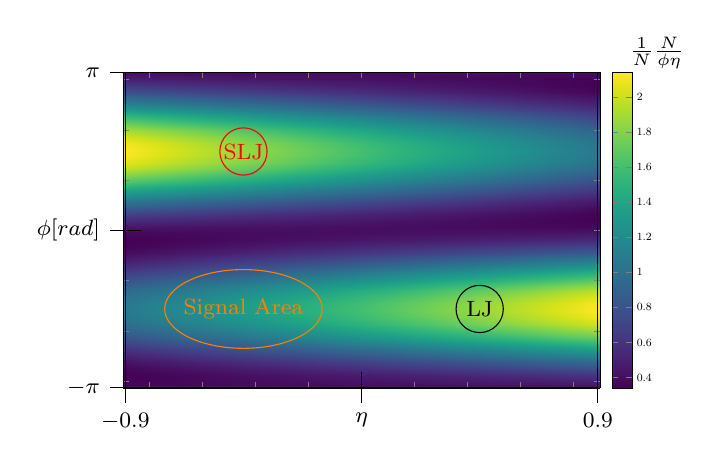
\begin{tikzpicture}[scale=0.5, every node/.style={font=\footnotesize}]
			
			\begin{axis}[
				height=9.6cm,
				width=13.7cm,
				font=\tiny,
				colorbar,
				anchor=center,
				view={0}{90},
				colormap/viridis,
				xlabel={},
				xticklabel=\empty,
				yticklabel=\empty,
				ylabel={},
				domain=-0.9:0.9,
				y domain=-3.14:3.14,
				samples=50,
				samples y=50,
				]
				
				\addplot3[
				surf,
				shader=interp,
				] {1+(-0.3*x)*2*cos(360*(y-3.14/2)/(2*3.14)) + 0.3*2*cos(720*(y-3.14/2)/(2*3.14))};
				
			\end{axis}
			
			%z label
			\node at (7.5,4.5) {$\frac{1}{N}\frac{\dif N}{\dif \phi \dif \eta}$};
			
			%phase spaces
			\draw[color=black] (-6.0,4.0) rectangle ++(12.0,-8.0);
			\draw (0, -3.6) -- (0, -4.4) node[below] {$\eta$};
			\draw (-6.0, -3.6) -- (-6.0, -4.4) node[below] {$-0.9$};
			\draw (6.0, -3.6) -- (6.0, -4.4) node[below] {$0.9$};
			\draw (-5.6, 0) -- (-6.4, 0) node[left] {$\phi \bunit{[rad]}$};
			\draw (-5.6, 4) -- (-6.4, 4) node[left] {$\pi$};
			\draw (-5.6, -4.0) -- (-6.4, -4.0) node[left] {$-\pi$};
			
			
			%background measurements
			\draw[color=orange] (-3,-2) ellipse (2cm and 1cm) node{Signal Area};
			\draw[color=red] (-3,2) circle (0.6) node{SLJ};
			\draw[color=black] (3.0,-2) circle (0.6) node{LJ};
			
			
		\end{tikzpicture}
	\end{minipage}
	\hfill
	\begin{minipage}[t]{0.48\textwidth}
		\centering
		\caption*{Small Gap}
		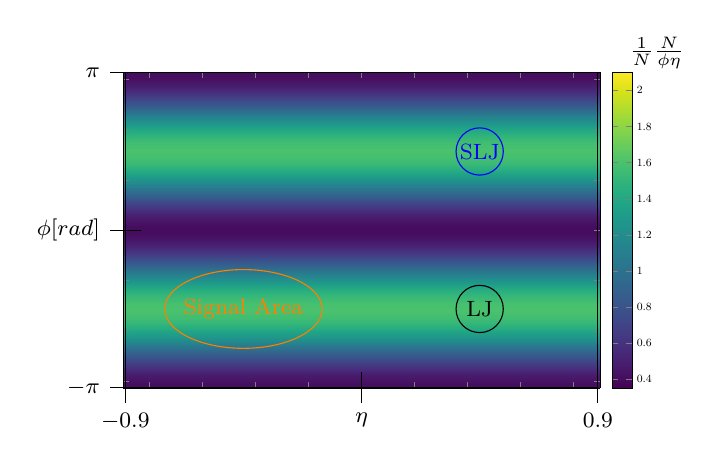
\begin{tikzpicture}[scale=0.5, every node/.style={font=\footnotesize}]
			
			\begin{axis}[
				height=9.6cm,
				width=13.7cm,
				font=\tiny,
				anchor=center,
				colorbar,
				point meta min=0.35,
				point meta max=2.1,
				view={0}{90},
				colormap/viridis,
				xlabel={},
				xticklabel=\empty,
				yticklabel=\empty,
				ylabel={},
				domain=-0.9:0.9,
				y domain=-3.14:3.14,
				samples=50,
				samples y=50,
				]
				
				\addplot3[
				surf,
				shader=interp,
				] {0.5*(1+(-0.3*x)*2*cos(360*(y+3.14/2)/(2*3.14)) + 0.3*2*cos(720*(y+3.14/2)/(2*3.14))) + 0.5*(1+(-0.3*x)*2*cos(360*(-y+3.14/2)/(2*3.14)) + 0.3*2*cos(720*(-y+3.14/2)/(2*3.14)))};
				
			\end{axis}
			
			%z label
			\node at (7.5,4.5) {$\frac{1}{N}\frac{\dif N}{\dif \phi \dif \eta}$};
			
			%phase spaces
			\draw[color=black] (-6.0,4.0) rectangle ++(12.0,-8.0);
			\draw (0, -3.6) -- (0, -4.4) node[below] {$\eta$};
			\draw (-6.0, -3.6) -- (-6.0, -4.4) node[below] {$-0.9$};
			\draw (6.0, -3.6) -- (6.0, -4.4) node[below] {$0.9$};
			\draw (-5.6, 0) -- (-6.4, 0) node[left] {$\phi \bunit{[rad]}$};
			\draw (-5.6, 4) -- (-6.4, 4) node[left] {$\pi$};
			\draw (-5.6, -4.0) -- (-6.4, -4.0) node[left] {$-\pi$};
			
			
			%background measurements
			\draw[color=orange] (-3,-2) ellipse (2cm and 1cm) node{Signal Area};
			\draw[color=blue] (3.0,2) circle (0.6) node{SLJ};
			\draw[color=black] (3.0,-2) circle (0.6) node{LJ};
			
			
		\end{tikzpicture}
		\caption*{Variant 1}
		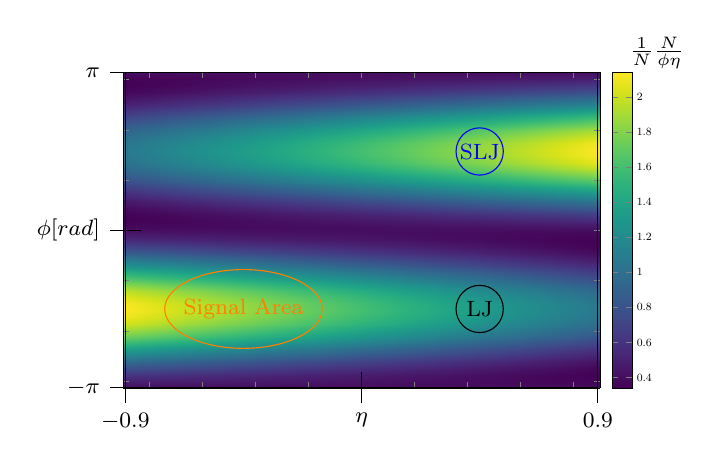
\begin{tikzpicture}[scale=0.5, every node/.style={font=\footnotesize}]
			
			\begin{axis}[
				height=9.6cm,
				width=13.7cm,
				font=\tiny,
				anchor=center,
				colorbar,
				view={0}{90},
				colormap/viridis,
				xlabel={},
				xticklabel=\empty,
				yticklabel=\empty,
				ylabel={},
				domain=-0.9:0.9,
				y domain=-3.14:3.14,
				samples=50,
				samples y=50,
				]
				
				\addplot3[
				surf,
				shader=interp,
				] {1+(-0.3*x)*2*cos(360*(y+3.14/2)/(2*3.14)) + 0.3*2*cos(720*(y+3.14/2)/(2*3.14))};
				
			\end{axis}
			
			%z label
			\node at (7.5,4.5) {$\frac{1}{N}\frac{\dif N}{\dif \phi \dif \eta}$};
			
			%phase spaces
			\draw[color=black] (-6.0,4.0) rectangle ++(12.0,-8.0);
			\draw (0, -3.6) -- (0, -4.4) node[below] {$\eta$};
			\draw (-6.0, -3.6) -- (-6.0, -4.4) node[below] {$-0.9$};
			\draw (6.0, -3.6) -- (6.0, -4.4) node[below] {$0.9$};
			\draw (-5.6, 0) -- (-6.4, 0) node[left] {$\phi \bunit{[rad]}$};
			\draw (-5.6, 4) -- (-6.4, 4) node[left] {$\pi$};
			\draw (-5.6, -4.0) -- (-6.4, -4.0) node[left] {$-\pi$};
			
			
			%background measurements
			\draw[color=orange] (-3,-2) ellipse (2cm and 1cm) node{Signal Area};
			\draw[color=blue] (3.0,2) circle (0.6) node{SLJ};
			\draw[color=black] (3.0,-2) circle (0.6) node{LJ};
			
			
		\end{tikzpicture}
		\caption*{Variant 2}
		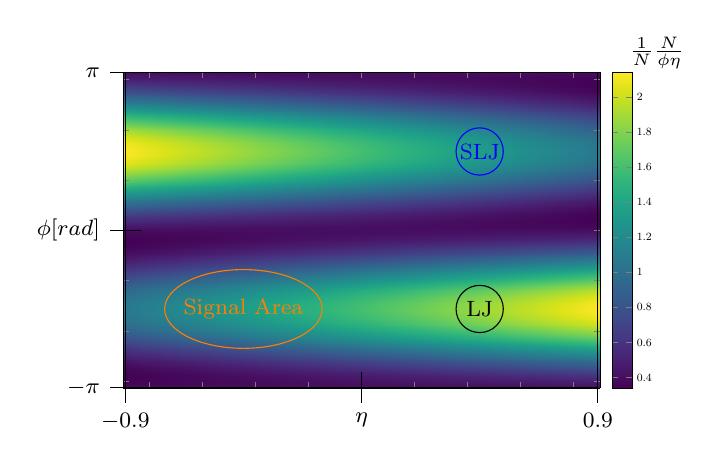
\begin{tikzpicture}[scale=0.5, every node/.style={font=\footnotesize}]
			
			\begin{axis}[
				height=9.6cm,
				width=13.7cm,
				font=\tiny,
				anchor=center,
				colorbar,
				view={0}{90},
				colormap/viridis,
				xlabel={},
				xticklabel=\empty,
				yticklabel=\empty,
				ylabel={},
				domain=-0.9:0.9,
				y domain=-3.14:3.14,
				samples=50,
				samples y=50,
				]
				
				\addplot3[
				surf,
				shader=interp,
				] {1+(-0.3*x)*2*cos(360*(-y+3.14/2)/(2*3.14)) + 0.3*2*cos(720*(-y+3.14/2)/(2*3.14))};
				
			\end{axis}
			
			%z label
			\node at (7.5,4.5) {$\frac{1}{N}\frac{\dif N}{\dif \phi \dif \eta}$};
			
			%phase spaces
			\draw[color=black] (-6.0,4.0) rectangle ++(12.0,-8.0);
			\draw (0, -3.6) -- (0, -4.4) node[below] {$\eta$};
			\draw (-6.0, -3.6) -- (-6.0, -4.4) node[below] {$-0.9$};
			\draw (6.0, -3.6) -- (6.0, -4.4) node[below] {$0.9$};
			\draw (-5.6, 0) -- (-6.4, 0) node[left] {$\phi \bunit{[rad]}$};
			\draw (-5.6, 4) -- (-6.4, 4) node[left] {$\pi$};
			\draw (-5.6, -4.0) -- (-6.4, -4.0) node[left] {$-\pi$};
			
			
			%background measurements
			\draw[color=orange] (-3,-2) ellipse (2cm and 1cm) node{Signal Area};
			\draw[color=blue] (3.0,2) circle (0.6) node{SLJ};
			\draw[color=black] (3.0,-2) circle (0.6) node{LJ};
			
			
		\end{tikzpicture}
	\end{minipage}
	\caption{The most probable correlations between the dijet pair and the soft hadron background in the large/small (left column / right column) gap case in the $(\phi, \eta)$ phase space. Soft hadrons are simulated with directed and elliptic flow with demonstration values $v_1 = -0.3\cdot \eta, v_2 = 0.3, \psi_m = \pi/2$. \textbf{LJ} are leading jets, \textbf{SLJ} are subleading jets. The region marked \textbf{Signal Area} is where the diffusion wake is expected. The large gap case only has one preferred dijet-soft hadron correlation. The small gap case has two variants in which jets compete for the soft hadron enhancement. The average is a mixture of the two variants.}
	\label{fig:v1Bias}
\end{figure}

To test the influence of the directed flow $v_1(\eta)$ on the analysis result its pseudorapidity dependency (equation (\ref{eq:simuparams})) is made bigger, so $v_1'(\eta) := M \cdot v_1(\eta)$.

Figure \ref{fig:flowresultsjet4020_V1Mag_100} shows the result of the dijet analysis using a transverse momentum threshold of $(40,20)\bunit{GeV/c}$ and a directed flow magnification of $M = 100$. The influence of the increased directed flow is strongest for the softest particles, decreasing with increasing transverse momentum bin. With the original directed flow configuration (figure \ref{fig:flowresultsjet4020_V1Mag_1}) the correlation difference with the $(40,20) \bunit{GeV/c}$ dijet trigger is non-zero but small. Increasing the directed flow leads to to a depletion of soft particles for $\eta < 0$ and an enhancement of soft particles for $\eta > 0$. To test the scalability of the effect another analysis with $M = 20$ is conducted. The result is shown in figure \ref{fig:flowresultsjet4020_V1Mag_20}. The directed flow effect competes with the bias found in the original flow configuration in figure \ref{fig:flowresultsjet4020}.

Figure \ref{fig:flowresultshad1510_V1Mag_100} shows the result of the dihadron analysis using a trigger hadron pair of $(15,10) \bunit{GeV/c}$ with a directed flow magnification of $M = 100$. The behavior is similar to the dijet trigger variant although the influence of the magnified $v_1'$ is smaller. The shape of the correlation difference for the softest particles coincides with the shape of the diffusion wake in the hydrodynamic prediction in figure \ref{fig:diffusionwakesimu}.

The comparison between the dijet and dihadron analysis in both cases, using the original flow $v_1$ and the magnified flow $v_1'$, has delivered interesting results. The signal opposing bias with the original $v_1$ is bigger for a dijet trigger than for a dihadron trigger. This is also the case when using a magnified $v_1'$. The influence is stronger when using dijets as triggers than using dihadrons. Since reconstructed jets are subject to bias through anisotropic flow (refer to section \ref{sec:analysis-of-heavy-ion-collision-data}), it is possible that these two effects are correlated.

\begin{figure}[H]
	\centering
	\includegraphics[width=\linewidth]{Media/Plots/FlowResults_Jet_40_20_V1Mag100.pdf}
	\caption{Results of the dijet analysis using simulated Pb--Pb data and leading/subleading jets with $(p_{T,\text{min}}^\text{Leading}, p_{T,\text{min}}^\text{Subleading}) = (40,20)\bunit{GeV/c}$ with a 100 times increased directed flow. $C_x = 1/N_x \cdot d N_x/d \eta$.	
		\textbf{(left)} Soft hadron correlations next to the leading jet for large gap and small gap events. \textbf{(right)} The differences between large gap and small gap correlations.}
	\label{fig:flowresultsjet4020_V1Mag_100}
\end{figure}

\begin{figure}[H]
	\centering
	\includegraphics[width=\linewidth]{Media/Plots/FlowResults_Jet_40_20.pdf}
	\caption{Results of the dijet analysis using simulated Pb--Pb data and leading/subleading hadrons with $(p_{T,\text{min}}^\text{Leading}, p_{T,\text{min}}^\text{Subleading}) = (15,10)\bunit{GeV/c}$ with the original directed flow. $C_x = 1/N_x \cdot d N_x/d \eta$.	
		\textbf{(left)} Soft hadron correlations next to the leading jet for large gap and small gap events. \textbf{(right)} The differences between large gap and small gap correlations.}
	\label{fig:flowresultsjet4020_V1Mag_1}
\end{figure}

\begin{figure}[H]
	\centering
	\includegraphics[width=\linewidth]{Media/Plots/FlowResults_Had_15_10_V1Mag100.pdf}
	\caption{Results of the dihadron analysis using simulated Pb--Pb data and leading/subleading hadrons with $(p_{T,\text{min}}^\text{Leading}, p_{T,\text{min}}^\text{Subleading}) = (15,10)\bunit{GeV/c}$ with a 100 times increased directed flow. $C_x = 1/N_x \cdot d N_x/d \eta$.	
		\textbf{(left)} Soft hadron correlations next to the leading jet for large gap and small gap events. \textbf{(right)} The differences between large gap and small gap correlations.}
	\label{fig:flowresultshad1510_V1Mag_100}
\end{figure}

\subsection{Simulating the azimuthal shift of reconstructed jets}

Two major effects influence the diffusion wake analysis when conducted with a dijet trigger.

In the selection of events for the diffusion wake analysis a dijet trigger above transverse momentum thresholds  $p_{T,\text{min}}^\text{Leading}$ and $p_{T,\text{min}}^\text{Subleading}$ is required \cite{yang_background-free_2025}. Since these thresholds are reached easier if the jet clustering is performed in the event plane, the dijet pair has a positive correlation with the event plane. Thus, events used for the diffusion wake analysis have their dijet pairs, on average, aligned with the event plane.

The second effect is important after the clustering has already brought the dijet pair above the $p_T$ thresholds. In section \ref{sec:hadron-triggers} it was mentioned that the behavior of jet clustering algorithms like the anti-$k_t$ algorithm depends on local quantities, like the underlying hadron density. The jet cluster algorithm weights the azimuthal coordinate of the cluster result based on the $p_T$ of each constituent \cite{cacciari_fastjet_2012}. This means that the leading hadrons of the jet define the final jet's position strongly. However, the underlying soft hadron constituents also contribute a fraction to the final position. Figure \ref{fig:jetshiftmodel} shows a gaussian profile of hard hadrons embedded in a low-$p_T$ hadron profile modulated with elliptic flow. Speaking in terms of figure \ref{fig:jetshiftmodel}, the average $p_T$ of the soft background hadrons to the left of the hard hadrons is higher than to the right. The non-uniform soft hadron background will therefore shift the final jet to the left compared to where the jet would have been clustered without the underlying background.

\begin{figure}[H]
	\centering
	\begin{tikzpicture}[scale=1.5]
		%draw coordinate system
		\draw [->] (-3.14,0) -- (3.14,0)node[right] {$\phi - \psi_m$ [rad]};
		\draw [->] (0,0) -- (0,3) node[above] {$\rho = \frac{d p_T}{d \phi}$};
		%draw functions
		\draw [red] plot[domain=-3.14:3.14,
		samples = 50,
		smooth]({\x}, {1 + 0.2*cos((360/6.28)*2*\x)});
		\draw [blue] plot[domain=-3.14:3.14,
		samples = 250]({\x}, {5*exp(-((\x-1)*(\x-1))/0.01)});
		%draw labels
		\draw (-3,3) node[color=red] {Background};
		\draw (-3,2.5) node[color=blue] {Hadron Jet};
		%draw arrows
		\draw[->, thick](1,1.5)--(0.5,1.5);
		
	\end{tikzpicture}
	\caption{The transverse momentum densities of the background (subject to elliptic flow) and of the hadron jet in azimuthal direction. The jet is produced independently of the underlying background. Because there are more soft hadrons to the left than to the right the jet clustered from PYTHIA+BG hadrons is more probably clustered farther left.}
	\label{fig:jetshiftmodel}
\end{figure}

A Pb--Pb event simulation as described in section \ref{sec:event-simulation} can be used to quantify how strongly the underlying soft background shifts the jet towards the event plane compared to where it would be clustered without any underlying background.

The jet clustering is first performed on a bare PYTHIA event that consists of jets but no soft hadron background to identify the leading jet with the properties $(\phi_{\text{Leading}}, \eta_{\text{Leading}}, p_{T,\text{Leading}})$. Next, the artificial soft hadron background is added to the PYTHIA event. The soft background is flow modulated and has a random event plane angle $\phi = \psi_m$. The leading jet has a distance of $d = \phi_{\text{Leading}} - \psi_m$ to the event plane. Now, another jet clustering is performed on the event, giving new information on the leading jet $(\phi'_{\text{Leading}}, \eta'_{\text{Leading}}, p'_{T,\text{Leading}})$. The shift $\Delta \phi = \phi'_{\text{Leading}} - \phi_{\text{Leading}}$ is studied depending on the original distance of the leading jet to the event plane $d$. 

\subsubsection{Modeling the jet shift}
\label{sec:modeling-jet-shift}

To be able to judge the result of the analysis, a simple model of the jet shift has to be introduced. Figure \ref{fig:jetshiftmodel} shows the overlay configuration of a jet and underlying soft hadron background that is subject to elliptic flow in the azimuthal direction. Due to symmetry reasons the shift is expected to be zero in the event plane or perpendicular to the event plane. The largest shift is expected if the soft hadron density asymmetry around the leading jet is greatest. Because the jet radius $R := 0.2$ is much smaller than the $v_2$ flow modulation spreads in azimuthal direction, the underlying flow can be expanded locally at the leading jet position according to

\begin{equation}
	\begin{gathered}
		\left. \rho_\text{BG}(\phi) \right|_{\phi_\text{Leading}} = \left. \frac{d p_T}{d (\phi - \psi_m)} \right|_{\phi_\text{Leading}} \propto \left. \frac{d N}{d (\phi - \psi_m)} \right|_{\phi_\text{Leading}} \\ \propto \left. 1 + 2 \sum_{n \geq 1}^{} v_n \cos(n (\phi - \psi_m)) \right|_{\phi_\text{Leading}}
		\stackrel{v_1 \ll v_2, v_n|_{n \geq 3} := 0}{\approx} \left. 1 + 2v_2 \cos(2(\phi - \psi_m)) \right|_{\phi_\text{Leading}}\\
		= \rho_0(\phi_\text{Leading}) + m \cdot (\phi - \phi_\text{Leading}) + \mathcal{O}(R^2) \text{ where } m \in \mathbb{R}
	\end{gathered}
	\label{eq:background_density}
\end{equation}

It is difficult to fully translate the anti-$k_t$ algorithm's behavior into an analytical model for many hadrons that are clustered. Therefore, the interest only lies in how the algorithm clusters a jet in the few-particle limit where only one high-$p_T$ jet hadron is clustered with one low-$p_T$ hadron in the thermal background. The position of the low-$p_T$ hadron is determined based on where it appears most probably around the jet hadron according to equation (\ref{eq:background_density}). This is sufficient to prove the first-order linear behavior of the jet shift $\Delta \phi$ in $m$.

\paragraph{Local coordinate system}

Since the jet clustering only happens in a small azimuthal range, it is appropriate to apply a small-angle approximation. The high-$p_T$ hadron, which is referred to as leading hadron for simplicity, has $\phi_\text{Leading} := 0$ and the soft hadron has the azimuthal coordinate $\phi_\text{h}$ (see figure \ref{fig:localcoord-shift}).

\begin{figure}[H]
	\centering
	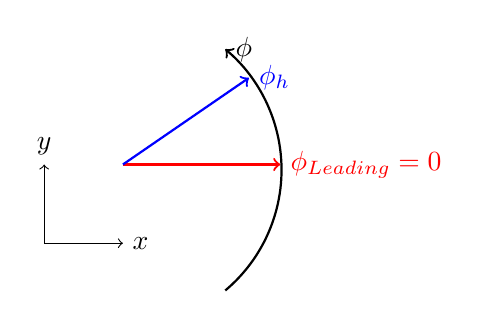
\begin{tikzpicture}
		
		% Particles
		\draw[thick , ->, red] (1,0) -- (3,0) node[right] {$\phi_\text{Leading} = 0$};
		\draw[thick , ->, blue] (1,0) -- (2.6,1.1) node[right] {$\phi_\text{h}$};
		
		% Winkelbogen oben
		\draw[thick, ->] (2.3,-1.6) arc[start angle=-50,end angle=50,radius=2] node[right] {$\phi$};
		
		% Kleines Koordinatensystem unten rechts
		\begin{scope}[shift={(0,-1)}]
			\draw[->] (0,0) -- (0,1) node[above] {$y$};
			\draw[->] (0,0) -- (1,0) node[right] {$x$};
		\end{scope}
		
	\end{tikzpicture}
	\caption{The ALICE coordinate system with the high-$p_T$ jet at $\phi = 0$ and the low-$p_T$ hadron at $\phi = \phi_h$.}
	\label{fig:localcoord-shift}
\end{figure}

Following this definition, the four-momenta of the leading hadron and the soft hadron are consequently

\begin{equation}
	\begin{gathered}
		p_\text{Leading}^\mu = (E_\text{Leading}, p_{T,\text{Leading}}, 0, 0), \\
		p_\text{h}^\mu = (E_\text{h}, p_{T,\text{h}} \cos(\phi_\text{h}), p_{T,\text{h}} \sin(\phi_\text{h}), 0) \stackrel{R \ll \text{Flow modulation}}{\approx} (E_\text{h}, p_{T,\text{h}} (1-\frac{\phi_\text{h}^2}{2}), p_{T,\text{h}} \phi_\text{h}, 0)
	\end{gathered}
	\label{eq:four-momenta-approximation}
\end{equation}

\paragraph{Clustering}

The anti-$k_t$ algorithm will cluster the leading hadron with the soft hadron by adding up their four-momenta such that the four-momentum of the resulting clustered jet is

\begin{equation}
	\begin{gathered}
		{p'}^\mu_{\text{Leading}} = p_\text{Leading}^\mu + p_\text{h}^\mu \stackrel{(\ref{eq:four-momenta-approximation})}{\approx} (E_\text{Leading} + E_\text{h}, p_{T,\text{Leading}} + p_{T,\text{h}}(1 - \frac{\phi_\text{h}^2}{2}), p_{T,\text{h}} \phi_\text{h}, 0) .
	\end{gathered}
\end{equation}

The azimuthal coordinate of the clustered jet $\phi'_\text{Leading}$ can be calculated from the four-momentum ${p'}^\mu_{\text{Leading}}$ using the geometric relation between ($\phi, p_x, p_y$)

\begin{equation}
	\begin{gathered}
		\phi'_\text{Leading} \approx \tan(\phi'_\text{Leading}) = \frac{{p'}^2}{{p'}^1} = \frac{p_{T,\text{h}} \phi_\text{h}}{p_{T,\text{Leading}} + p_{T,\text{h}} (1-\frac{\phi_\text{h}^2}{2})} \stackrel{\phi_\text{h}^2 \ll R}{\approx} \frac{p_{T,\text{h}} \phi_\text{h}}{p_{T,\text{Leading}} + p_{T,\text{h}} } \propto \phi_\text{h}
	\end{gathered}
\end{equation}

\paragraph{The soft hadron's position}

The BG particle is generated based on $\rho_{BG}(\phi)$ in proximity to the jet within a jet radius $R$. The expected coordinate of the BG particle can be calculated according to

\begin{equation}
	\begin{gathered}
		<\phi_\text{h}> = \frac{\int_{-R}^{R} d\phi \, \phi \, \rho_{BG}(\phi)}{\int_{-R}^{R} d\phi \,  \rho_{BG}(\phi)} \stackrel{(\ref{eq:background_density})}{\propto} \int_{-R}^{R} d\phi \, \phi \, (\rho_0 + m \phi + \mathcal{O}(R^2)) = \frac{2}{3} m R^3 + \mathcal{O}(R^4) \propto m
	\end{gathered}
\end{equation}

\paragraph{Conclusion}

Thus, it can be concluded that

\begin{equation}
	\begin{gathered}
		<\phi'_\text{Leading}> \propto <\phi_\text{h}> \propto m = \left. \frac{d \rho_{BG}(\phi)}{d \phi} \right|_{\phi_\text{Leading}} = - 4 v_2 \sin(2(\phi_\text{Leading} - \psi_m))
	\end{gathered}
\end{equation}

and the final shift can be modeled with

\begin{equation}
	\begin{gathered}
		<\Delta \phi> = <\phi'_\text{Leading} - \phi_\text{Leading}> = A \sin(2(\phi_\text{Leading} - \psi_m)) = A \sin(2 d)
	\end{gathered}
\end{equation}

where $A$ is a fit parameter.

\subsubsection{Jet shift in simulated Pb-Pb events}

\begin{figure}[H]
	\centering
	\includegraphics[width=\linewidth]{Media/Plots/JetShiftResult.pdf}
	\caption{The shift of reconstructed jets towards the event plane in simulated Pb--Pb events.}
	\label{fig:jetshiftresult}
\end{figure}

Figure \ref{fig:jetshiftresult} shows the fitted results for the shift of reconstructed jets towards the event plane in simulated Pb--Pb events. The results are presented separately for different jet transverse momentum bins. The categorization is made before adding the soft hadron background. The general shape of the histogram resembles the expectations. Speaking in terms of figure \ref{fig:jetshiftmodel}: If the jet is right of the event plane, it gets pulled to the left and vice versa. As expected, soft jets are pulled stronger than hard jets because for harder jets an individual soft hadron contributes a smaller fraction to the total jet than for soft jets. The softest jets with $20.0 \leq p_{T,\text{Leading}} \leq 40.0 \bunit{GeV/c}$ are pulled by a maximum value of $d = 1.458 \cdot 10^{-2} \bunit{rad} = 0.836 \deg$. The jets are pulled hardest if they are approximately located where the local azimuthal elliptic flow changes the greatest, i.e. for $d = \pm \pi/4$. The fit model derived in \ref{sec:modeling-jet-shift} approximately resembles the measured behavior, but does not fully explain the result. The shift tends to be greatest slightly off of $d = \pm \pi/2$. Reasons for this behavior could be truncation errors in the model derivation or that the linear behavior of the jet algorithm in the single particle approximation breaks down too quickly for more particles.



\iffalse

\subsection{Single hadron analysis with MC events}


The measurement of the diffusion wake in a dijet-hadron correlation or a dihadron-hadron correlation is done to isolate the diffusion wake signal from the uncorrelated soft background. Naively one could think about selecting evens that have a single high-$p_T$ hadron and to study the correlation of soft hadrons with the trigger hadron. If the trigger hadron has an azimuthal coordinate $\phi_\text{trigger}$, its diffusion wake and therefore the soft hadron depletion is expected at $\phi_\text{depletion} =  \phi_\text{trigger} \pm \pi$. Therefore the soft soft hadron correlation is studied azimuthally opposite in the full pseudorapidity range, that is $|\phi_\text{depletion} - \phi_h| < \Delta \phi, -0.9 \leq \eta_h \leq 0.9$ where $\Delta \phi$ defines how far soft hadrons are allowed to be from the depletion site to be studied. This correlation has to be interpreted relative to another soft hadron correlation that is unbiased by the trigger hadron. To avoid acceptance and tracking efficiency effects this reference correlation should be studied exactly where the original correlation is studied in the $(\phi, \eta)$ phase space. One possibility to accomplish that is to choose a reference event that has similar properties like the original event. Events are defined to be similar if their particle multiplicity and event plane angle are similar. The reference event only differs from the original event by not having a hard hadron where the trigger hadron in the original event was. Then the reference region is uncorrelated to the trigger hadron in the original event. By subtracting the reference correlation from the soft hadron correlation behind the trigger hadron one should be able to isolate its influence on the soft particle spectrum.

The analysis is conducted as follows. At once around 2000 events are analyzed simultaneously. Each of the events is first checked for a trigger hadron above some threshold, just like in the dijet analysis. Then the azimuthally opposite side of this trigger hadron, where the soft hadron correlation is measured, is required to be free of any high-$p_T$ objects within $\Delta \phi$. If an event fulfills these requirements it is considered suitable for the single hadron analysis. Then, a suitable reference event is chosen for each event. The reference event must have a particle multiplicity that is not far off the original multiplicity, i.e. $|N_i - N_\text{reference(i)}| < \Delta N$ and a similar event plane angle, i.e. $|\psi_{m,i} - \psi_{m,\text{reference(i)}}| < \Delta \psi$. Azimuthally it must also be free of any high-$p_T$ objects around the original trigger hadron in event $i$ and around its azimuthally opposite side within $\Delta \phi$. 

If an event fulfills these requirements it is considered a suitable reference event of event $i$.

When choosing to study a low-$p_T$ spectrum of soft hadrons that are azimuthally opposite to the trigger hadron the diffusion wake should manifest itself as a dip in the particle spectrum at low transverse momenta. 

\fi


\end{document}